% Set the author and title of the compiled pdf
\hypersetup{
  pdftitle = {\Title},
  pdfauthor = {\Author}
}

% Lecture 1

\section{Intro}

A compiler is a program that reads another program written in one language and
translates it into an equivalent program written in another language.

An interpreter reads the source code of a program and produces the results of
executing the source. Many issues related to compilers are also present in the
construction and execution of interpreters.

A good compiler exhibits the following qualities:

\begin{itemize}
  \item It generates correct code
  \item It generates code that runs fast
  \item It confirms to the specification of the input language
  \item It copes with any input size, number of variables, line length etc
  \item The time taken to compile source code is linear in its size
  \item It has good diagnostics
  \item It has \textit{consistent} optimisation's
  \item It works will with a debugger
\end{itemize}

An example of a compiler that optimises code is if we had a for-loop such as:

\begin{verbatim}
  A = []
  for i = 0 to N:
    A[i] = i
  endfor
\end{verbatim}

If \texttt{N} was always equal to \texttt{1}, then the compiler should optimise
this to:

\begin{verbatim}
  A = [1]
\end{verbatim}

There are two things that any sensible compiler \textit{must} do:

\begin{itemize}
  \item Preserve the meaning of the program being compiled
  \item Improve the source code in some way
\end{itemize}

In addition, it could do some (it's pretty much impossible to do all) of these
things:

\begin{itemize}
  \item Make the output code run fast
  \item Make the size of the output code small
  \item Provide good feedback to the programmer; error messages, warnings etc
  \item Provide good debugging information (this is hard since transforming the
  program from one language into another often obscures the relationship between
  an instance of a program at runtime and the source code it was derived from).
  \item Compile the code quickly
\end{itemize}

% Lecture 2

\section{Parts of the compiler}

In this section, we'll give a brief overview of all the bits inside a compiler.
Most compilers can be roughly split into two parts; the front end and the back
end:

\begin{description}
  \item The front end is concerned with analysis of the source language, making
  sure that the input is legal and producing an intermediate representation.
  \item The back end translates the intermediate representation into the target
  code. This usually involves choosing appropriate instructions for each 
  operation in the intermediate representation.
\end{description}

Usually, the front end can run in linear time, while the back end is
\texttt{NP-Complete}. We cam automate much of the front end of the compiler.

Having an intermediate representation (IR) of the program is so helpful since it
means we can completely separate the front and back ends of a compiler.
Consequently, we can have multiple front ends all compiling different languages
into the same IR, and multiple back ends producing instructions for different
architectures.

If we have $n$ languages and $m$ architectures, then we'd need to write $n
\times m$ monolithic compilers, but can instead write $n$ front ends and $m$
back ends ($n+ m$). This is \textit{almost} as good as it sounds; in practice,
you need to choose your IR very carefully, since its hard to make it encapsulate
everything all the features of a language (a good example of this is compiling
Scala onto code that runs on the JVM, where type erasure is a big limitation for
Scala).

In more detail, we code goes through the following steps inside the compiler:

\begin{description}
  \item \textbf{Lexical Analysis} (front end):\\
  Here, the source language is read in and tokenized (grouped into tokens for 
  later). If the input was \texttt{a = b + x}, you might get
  \texttt{(id,a)(=)(id,b)(+)(id,c)} out of the other end. Whitespace is usually
  ignored (or, depending on the language, Incorporated into the parsing), and
  a symbol table is generated, containing the words that are not reserved words
  in the language (e.g. variable names).

  \item \textbf{Syntax Analysis} (front end):\\
  Here, the tokens are given a hierarchical structure, often using recursive
  rules such as Context Free Grammars. The output might be an \textbf{Abstract
  Syntax Tree} (AST), which is an abstract representation of the program
  (basically an IR).

  \item \textbf{Semantic Analysis} (front end):\\
  Here, we check for semantic errors (such as type checking, flow control
  checks etc). The AST is annotated with the results of the checks which can be
  used for optimisation later.

  \item \textbf{Intermediate code generation} (front end):\\
  The AST is now translated into the IR. If the AST is constructed well, and IR
  is well chosen, then this should be fairly straightforward. Three address code
  might be an example of an IR.

  \item \textbf{Optimisation} (back end):\\
  The IR is now optimised to increase how quickly it runs, or decrease how much
  space it uses etc. Some optimisation are easier than others, and some are
  very complex! Often, the optimisation stage is so complex, that it could be
  a whole separate part of the compiler (a middle stage in-between the front and
  back ends).

  \item \textbf{Code generation} (back end):\\
  This phase is concerned with things such as register allocation (NP-Complete),
  instruction selection (pattern matching), instruction scheduling (NP-Complete)
  and more. Architecture specific information may be used for further
  optimisation here, and machine code is the output.
\end{description}

% Lecture 3

\section{Lexical Analysis}

So, lexical analysis is where we read the characters in the input and produce a
sequence of tokens (i.e. tokenize the input). We want to do this in an automatic
manner.

When translating from a programming language or a natural language, we need to
map words to parts of speech. In programming languages, this is syntactic (as
opposed to being idiosyncratic in natural languages), and is based on notation.
Things like reserved words are very important in tagging a programming language.

To talk about lexical analysis, we should make some definitions:

\marginpar{See my computation notes (\texttt{COMP11212}) for more on CFG's}

\begin{itemize}
  \item A vocabulary (or alphabet) is some finite set of symbols.
  \item A String is a finite sequence of symbols from the vocabulary.
  \item A Context Free Grammar (CFG) is a 4-tuple; $(S,N,T,P)$:
    \begin{itemize}
      \item $S$: The starting symbol.
      \item $N$: The non-terminal symbols.
      \item $T$: The set of terminal symbols.
      \item $P$: A set of production rules.
    \end{itemize}
  \marginpar{Terminal symbols will usually start with a lower case letter, and
  non-terminal symbols will start with an upper case one.}
  \item A Language is any set of strings over a fixed vocabulary, or the set of
  terminal productions of a CFG. 
\end{itemize}

We can use repeated substitution to derive \textit{sentinel forms}.
% See notes for example

Leftmost derivation is when the leftmost non-terminal symbol is expanded at each
step. When we're recognising a valid sentence, we reverse this process.

%TODO: Try example on page 4 of lecture 3.

If we have a knowledge about lexical analysis, we can avoid having to write a
lexical analyser by hand, and can simplify the specification and implementation
of a language. We need to specify a \textit{lexical pattern} to derive tokens,
which is essentially a CFG.

Some parts of this are easy, for example:

\[
  \text{WhiteSpace} \rightarrow \text{blank} | \text{tab}
    | \text{WhiteSpace blank} | \text{WhiteSpace} tab
\]

Things like keywords, operators and comments are easy to use as well. However,
some parts of languages are more complicated, such as identifiers and numbers.
We want a notation that lets us go easily to an implementation.

Regular expressions are a way of specifying a regular language; they are
formulas that represent a possibly infinite set of strings. A Regular Expression
(RE) over the vocabulary $V$ is defined as:

\begin{itemize}
  \item $\epsilon$ is a RE denoting the empty set.
  \item If $a \in V$ then $a$ denotes $\{a\}$.
  \item If $r_1$ and $r_2$ are RE's, then:
  \begin{itemize}
    \item $r^{*}_1$ denotes zero or more occurrences of $r_1$
    \item $r_1r_2$ denotes concatenation
    \item $r_1|r_2$ denotes either or.
  \end{itemize}
  \item Short-hands include $[a-d]$ which expands to $[a|b|c|d]$, $r^+$ for
  $rr^*$ and $r?$ for $[r|\epsilon]$
\end{itemize}

%TODO: What languages cannot be described by regular expressions?

Building a lexical analyser by hand may involve a function with lots of if/else
statements as we try to classify each character one by one.

A different idea is to try and match the input to different regular expressions
and use the one with the longest match. This would be linear in the number of
regular expressions we have (we would need to do a fresh search for each). 
%See slide 9 of lecture 3

We could study the regular expressions we have and try to automate the
construction of a scanner. Some regular expressions can be converted into
transition diagrams. For example, matching a register ($r(0-9)+$) can be
converted to the following:

% TODO: Insert transition diagram here

The regex would accept the string if the transition diagram ends in an accept
state after the string has been run through it. We can produce a transition
table (one way of encoding automata in computers) and (once we've figured out
how to produce the table, which we'll soon find out) run through the input
string in linear time.

% Lecture 4

\subsection{Deriving a Deterministic Finite Automata from a Regular Expression}

\marginpar{Remember that a DFA is a special case of an NFA.}

Every regular expression can be converted to a deterministic finite automaton
(DFA), and DFA's can automate lexical analysis.

For example, the regular expression describing CPU registers (0-31) could be:

\[
  \text{Register} \rightarrow
    r((0|1|2)(\text{Digit}|\epsilon)|([4-9])|(3|30|31))
\]

 % TODO: Reproduce transition table from notes.

If we generated the DFA shown in Figure~\ref{fig:DFA-1}, we could produce a
transition table like:

\begin{center}
  \begin{tabular}{>{$}c<{$}|>{$}c<{$} >{$}c<{$} >{$}c<{$} >{$}c<{$} >{$}c<{$}}
    State & r & 0,1 & 2 & 3 & 4 \dots 9\\ \hline
    0     & 1 & -   & - & - & -\\
    1     & - & 2   & 2 & 5 & 4\\
    2(fin)& - & 3   & 3 & 3 & 3\\
    3(fin)& - & -   & - & - & -\\
    4(fin)& - & -   & - & - & -\\
    5(fin)& - & 6   & - & - & -\\
    6(fin)& - & -   & - & - & -\\
  \end{tabular}
\end{center}

This is done by creating an NFA for each thing you can do in a regular
expression (concatenation, either operator, star operator etc) and putting them
together.

% Example of creating an NFA from a RE

Converting a RE into an NFA is more direct, but its also a lot slower to parse
(since NFA's can have many paths through them). Converting to a DFA is slower
(and the resulting automata is slower), but lets us parse an input in linear
time.

The idea is:

\marginpar{That's Ken Thompson, the guy who wrote unix.}

\begin{enumerate}
  \item Write down the RE for the input language
  \item Convert it to an NFA (Thompson's construction)
  \item Build a DFA to simulate the NFA (subset construction)
  \item Shrink the DFA (Hopcroft's algorithm)
\end{enumerate}

%TODO: Include NFA's from slide 5 of lecture 4

%TODO: Construct the NFA of a(b|c)* 

We have seen the subset construction algorithm before (in \text{COMP11212}),
where it was called `Algorithm One'. There is a rather compact but (I think)
working implementation in \texttt{COMP36512/programs/nfa-dfa.py} on Github that
you could look at.

Before we look at the algorithm itself, we need to look at two operations:

\begin{description}
  \item \texttt{move(states, a)} Returns all the states to which there is a
  transition from some state in \texttt{states} with the symbol \texttt{a}.
  \item \texttt{e-closure(states)} All the states that are reachable using only
  epsilon transitions from any state in \texttt{states}.
\end{description}

The algorithm is:

\begin{lstlisting}
  dStates = e-closure(startState)
  markedStates = []
  dTable = {}
  // While there are unmarked states
  while (dStates - markedStates) is not []:
    t = (dStates - markedStates).get(0)
    markedStates.add(t)
    for symbol in alphabet:
      U = e-closure(move(t, symbol))
      if U in dStates:
        dStates.add(U)
      dTable(t, a) = U
\end{lstlisting}

This builds up a table (representing a DFA) by creating states representing all
the states reachable with a specific symbol from a set of states within the NFA.

%TODO: Example of NFA->DFA

% Lecture 5

\subsection{DFA minimisation; Hopcroft's algorithm}

The main disadvantage of DFA's is that they can be rather large (when converting
from an NFA to a DFA, the DFA could have worst case exponential number of
states). As a result, Hopcroft's algorithm for minim sing the number of states in
a DFA is good for our memory usage.

The idea behind the algorithm is to find groups of states where for each input
symbol, every state in the group will have transitions exclusively within the
group.

The algorithm is:

\begin{verbatim}
  while the groups are not stable {
    for each group g {
      for each input symbol I {
        for each state s in g {
          if s(g) not in g {
            put s in its own group
          }
        }
      }
    }
  }
\end{verbatim}

%TODO: Include example from slide 4 of lecture 5


\subsection{Fast scanners}

Now it is very easy to build a recogniser for the DFA, we can just get the
transition table for the DFA, and read each character of the input,
transitioning to the next state every time. Accepting and rejecting depends on
whether we get to \texttt{eof} in a finishing state (accept )or we didn't/we
made an invalid transition (reject).

However, table recognisers aren't as fast as they could be; each character
requires one memory access, which is not very efficient, especially if the
transition table is big and won't fit in a cache. Some automatic code generation
tools will output a series of \texttt{goto} or \texttt{case} statements instead,
since then a transition table isn't needed (the states are hardcoded into the
program).

Poor language design can complicate analysis though. For example, in Fortran:

\begin{verbatim}
  DO5i=1,25
    ...
  5
\end{verbatim}

Is a for-loop from 1 to 25. However, the following is also valid:

\begin{verbatim}
  DO5i=1.25
    ...
  5
\end{verbatim}

\marginpar{This may not exactly be what happens, but it's the thought that
counts.}

The only difference is that there is a comma instead of a period, but now the
compiler will have assigned the token \texttt{DO5i} a value of $1.25$, and the 5
at the end will be a non-operation.

Similarly, in C++ having types within types can be hard since
\texttt{myType<myType2<int>>} includes the symbols \texttt{>>}, which is the
operator for writing to an output stream.

%Slide 10.. expand :P
\texttt{lex} and \texttt{flex} are tools for generating lexical analysers.

% Lecture 6

% No content; questions lecture

% Lecture 7

\section{Parsing languages}

Not all languages can be described by regular expressions (as we have attempted
to do so far). They cannot describe things like nested constructs (i.e. is the
bracketing legal in a mathematical formula). Also, you can't use a terminal
symbol in a regular expression before it has been fully defined (i.e. no
recursion).

Chomsky's hierarchy of grammars tells us which grammars can describe other ones:

\begin{description}
  \item \textbf{Phase structured}: % TODO phase structured example
  \item \textbf{Context sensitive}: % TODO CSG example
  \item \textbf{Context free}: % TODO CFG example
  \item \textbf{Regular}:\\
    Only rules of the form $A \rightarrow \epsilon$, $A \rightarrow a$,
    $A \rightarrow pB$ are allowed.  % TODO regex example
\end{description}

Context free syntax is expressed with a context free grammar, which is a 4-tuple
$G = \{S,N,T,P\}$, where $S$ is the start symbol, $N$ are the non-terminal
symbols, $T$ are the terminal symbols and $P$ are the production rules. We re-
write rules (starting from the initial rule) in order to make them closer to a
sentence we're trying to obtain. A sequence of re-writes leading to some desired
output is called a \textit{derivation}, and the process of finding a derivation
for a specific sentence is called \textit{parsing}.

A derivation is a sequence of steps from the initial rule to a parsed
representation of the input. Different choices of steps can potentially lead to
different derivations of the same input. Two derivations are of particular
interest to us:

\begin{description}
  \item Leftmost derivation; at each step, replace the leftmost non-terminal.
  \item Rightmost derivation; at each step, replace the rightmost non-terminal.
\end{description}

A parse tree is a graphical representation of a derivation that is independent
of the order that the derivation rules were applied in. To construct a parse
tree, start with the starting symbol (which is the root of the tree), then for
each derivational step, add children nodes for each symbol on the right hand of
the production rule to the node for the left side. After you've done this, the
leaves of the tree will (should) read from left to right to form the input.

If we're parsing something like a mathematical formula, then we need to build
the notion of precedence into our derivational rules so that we get the correct
parsing for an input. To do this, we force the parser to recognise the high-
precedence subexpressions first.

Grammars are ambiguous if they can possibly produce more than one parse tree for
a sentence. This is the case if a grammar has more than one leftmost or
rightmost derivation for a single sentinel form. An example is:

\begin{verbatim}
  Stmt = if Expr then Stmt | if Expr then Stmt else Stmt | Expr
  Expr = W | X | Y | Z
\end{verbatim}

This could match the following in two ways:

\begin{verbatim}
  if X then if Y then W else Z
\end{verbatim}

In order to eliminate ambiguity (and also deal with precedence), we need to re-
write the grammar:

%TODO: Lecture 7 S 8, does this even work?! HMMMMM
\begin{verbatim}
  Stmt = IfElse | IfNoElse
  IfElse = if Expre then IfWithElse else IfWithElse
  IfNoElse = if Expr then Stmt | if Expr then IfElse else IfNoElse
  Expr = W | X | Y | Z
\end{verbatim}

So, if there is ambiguity, then we should try and resolve it in the CFG (after
all, we only have to do this once, instead of resolving at runtime every time!).
Overloading (when you give multiple things the same name or structure, such as
method overloading in Java) can create ambiguity that you can only resolve using
context. In general, to solve ambiguity:

\begin{description}
  \item If the issue is context free, then re-write the CFG so that there is no
  ambiguity.
  \item If the issue requires context to solve, then we need more information
  in order to continue. This is really a problem with the design of the
  language.
\end{description}

There are two broad classes of parsers; top down parsers and bottom up parsers:

% TODO: Research these more
\begin{description}
  \item \textbf{Top-down parsers}:\\
    \begin{itemize}
      \item Construct the root of the tree first, then construct the rest in
      pre-order, using a depth first search.
      \item Pick a production, and try to match the input. If you fail then use
      backtracking.
      \item Try to find a leftmost derivation for the input string where we scan
      from left to right.
      \item Some grammars are backtrack-free (called predictive parsing)
    \end{itemize}
  \item \textbf{Bottom-up parsers}:\\
    \begin{itemize}
      \item Construct the tree for an input but start at the leaves and work up
      towards the root.
      \item Use a left-to-right scan and try to construct a rightmost derivation
      in reverse.
      \item Handles a large number of grammars.
    \end{itemize}
\end{description}

% Lecture 8

\subsection{Top Down Recursive Descent Parsing}

This is where you:

\begin{itemize}
  \item Construct the root with the start symbol for the grammar
  \item While the leaves of the parse tree don't match the input:
  \begin{itemize}
    \item Select a node in the tree labelled $A$.
    \item Select a production rule for $A$ and construct a child for each symbol
    on the right hand side of the rule.
    \item When a terminal symbol is added to the fringe, but it doesn't match
    the fringe, then backtrack.
  \end{itemize}
\end{itemize}

If you choose the right production step at each stage, then this algorithm is
fast, if you don't then the runtime will increase due to backtracking.

A grammar is left-recursive if it has a non-terminal symbol $A$ such that there
is a derivation $A \rightarrow Aa$ for some string $a$. Such a grammar can cause
an infinite look for recursive-descent parsers since they may output an string
of infinite $a$'s. To avoid this, we try to eliminate left recursion; i.e.
replace $A \rightarrow Aa | b$ with $A \rightarrow bA$ $A' \rightarrow aA' |
\epsilon$.

The general algorithm for non-cyclic, non-$\epsilon$-productive grammars is:

\begin{itemize}
  \item Arrange the non-terminal symbols $A_1 \dots A_n$
  \item For $i = 1 \dots n$:
    \begin{itemize}
      \item For $j = 1 \dots i-1$:
      \begin{itemize}
        \item Replace each production $A_i \rightarrow A_j \gamma$ with
        $A_I \rightarrow \delta_1 \gamma | \dots | \delta_k\gamma$, where
        $A_j \rightarrow \delta _1 | \dots | \delta_k$ are the current $A_j$
        productions.
        \item Eliminate the left recursion among $A_i$.
      \end{itemize}
    \end{itemize}
\end{itemize}

\subsubsection{Predictive parsing}

So now we can make a top-down parser which will find the correct matching in
finite time, but it employs backtracking when it picks the wrong initial rule
(which slows everything down). If we look ahead in the input, we can use context
to influence our decisions about what production rules to try next so we can
attempt to reduce the amount we have to backtrack.

In general, we need an infinite amount of look-ahead to always make the right
decision about what production rule to use next (but this is pretty much the
same as parsing the rest of the string, right?). However, most context free
grammars can be parsed with a limited look-ahead.

The basic idea is for any production $A \rightarrow a | b$, we want to have a
distinct way of choosing the correct production to expand (either $a$ or $b$).

We can do this for some grammars by defining a set called \texttt{FIRST}. This
is the set of the first terminal symbols for each string derived from $A$. A
very simple example is:

\[
  A \rightarrow B | C
\]

\[
  B \rightarrow x | y
\]

\[
  C \rightarrow m | n
\]

\[
  FIRST(B) = \{x, y\}
\]

\[
  FIRST(C) = \{m, n\}
\]

% TODO: What's the LL property?

If for a production rule $A \rightarrow X | Y$, $FIRST(X) \cap FIRST(Y) =
\emptyset$, then we can implement the look-ahead with only one symbol. This is
the LL property.

If a grammar does not have the LL(1) property, we can sometimes transform it so
that it does:

\begin{itemize}
  \item For each non-terminal $A$, find the longest prefix $a$ common to two or
  more of its alternatives (e.g. $B$ and $C$ in $A \rightarrow B | C$).
  \item If $a \neq \epsilon$ then replace all the $A$ productions
  $A \rightarrow ab_1 | \dots | ab_n | \gamma$ (where $\gamma$ doesn't begin
  with $a$) with $A \rightarrow aZ | \gamma, Z \rightarrow b_1 | \dots b_n$.
  \item Repeat until we have no common prefixes.
\end{itemize}

% TODO: Give example

Note that it is undecidable as to whether an LL(1) grammar exists for any CFG.
It is also possible to parse non-recursively if we maintain a stack and
determine what production rules to apply using a table.

% Lecture 9

\subsection{Bottom up parsing}

The goal for bottom-up parsing is the same as that of top-down parsing;
construct a parse tree for a string $s$ given some grammar $G$. Bottom-up
parsing starts from the string and works back towards the start symbol of the
grammar, whereas top-down goes the other way.

Bottom-up parsing works by applying a sequence of reductions to the input
string. A reduction corresponds directly to a rule in the input grammar, and
takes the form $A \rightarrow b$.

If we defined our grammar $G$ to be:

\begin{center}
  \begin{tabular}{r >{$}c<{$}}
    1. & S \rightarrow LMR\\
    2. & L \rightarrow c\\
    3. & M \rightarrow Mo | o\\
    4. & R \rightarrow mpilers
  \end{tabular}
\end{center}

We could parse input like so:

\begin{center}
  \begin{tabular}{|c|c|c|}
    \hline
    Sentinel Form & Production & Position\\ \hline
    cooooompilers   & 2          & 1\\
    LMoooompilers   & 3          & 2\\
    LMooompilers    & 3          & 3\\
    LMoompilers     & 3          & 3\\
    LMompilers      & 3          & 3\\
    LMmpilers       & 3          & 9\\
    LMR             & 4          & 3\\
    S               & -          & -\\ \hline
  \end{tabular}
\end{center}

To do the above, we needed to find some substring $s_1$ that could match the
right side of a production that would occur in the rightmost
derivation\footnote{As if we started from the start-state of the grammar and
always expanded the rightmost non-terminal.} To be able to reason about this, we
define a handle, which is a pair $(A \rightarrow b, k)$, where $A \rightarrow b
\in G$ and $k$ is the position in the input string of the \textit{rightmost} symbol in
$b$.

This is efficient because since we're dealing with a right sentential form,
anything to the right of the handle is a terminal symbol, meaning the compiler
doesn't have to scan past the handle.

\subsubsection{Shift reduce parsers}

A basic bottom-up, shift reduce parser is stack based and has four operations:

\begin{description}
  \item \textbf{Shift}: The next input is shifted onto the top of the stack.
  \item \textbf{Reduce}: The right end of the handle is on the top of the
  stack. Locate the left end of the handle within the stack\footnote{You can
  just keep popping until you reach the end of the handle}, pop the handle of
  the stack and push the appropriate non-terminal symbol.
  \item \textbf{Accept}: The string was parsed successfully.
  \item \textbf{Error}: Handle the error somehow (implementation dependent).
\end{description}

Using the `cooooompilers' example again:

% TODO: Check this
\begin{center} 
  \begin{tabular}{|l|r|c|c|}
    \hline
    Stack & Input         & Handle & Action\\ \hline
    \$    & cooooompilers & None   & Shift\\
    \$c   & ooooompilers  & 2, 1   & Reduce 2\\
    \$L   & ooooompilers  & None   & Shift\\ 
    \$Lo  & oooompilers   & 3, 2   & Reduce 3\\
    \$LM  & oooompilers   & None   & Shift\\
    \$LMo & ooompilers    & 3, 3   & Reduce 3\\
    \$LM  & ooompilers    & None   & Shift\\
    \$LMo & oompilers     & 3, 2   & Reduce 3\\
    \$LM  & oompilers     & None   & Shift\\
    \$LMo & ompilers      & 3, 2   & Reduce 3\\
    \$LM  & ompilers      & None   & Shift\\
    \$LMo & mpilers       & 3, 2   & Reduce 3\\
    \$LMm & pilers        & None   & Shift\\
    \$LMmp & ilers        & None   & Shift\\
    \$LMmpi & lers        & None   & Shift\\
    \$LMmpil & ers        & None   & Shift\\
    \$LMmpile & rs        & None   & Shift\\
    \$LMmpiler & s        & None   & Shift\\
    \$LMmpilers &         & 4,9    & Reduce 4\\
    \$LMR       &         & 4,9    & Reduce 4\\
    \$G         &         & None   & Accept\\ \hline
  \end{tabular}
\end{center}

There are two possible things that can go wrong here:

\begin{description}
  \item \textbf{Shift/Reduce conflict}: The parser can't decide whether to do 
  a shift or a reduce. This is usually because of an ambiguous grammar. The 
  solution is to make the grammar unambiguous or just always choose shift.
  \item \textbf{Reduce/Reduce conflict}: The parser can't decide which (of 
  several) reduction to make.
\end{description}

\subsubsection{LR parsers}

If we want to avoid reduce/reduce conflicts, then we need to have a
\texttt{LR(1)} grammar. This is a grammar where we can always choose the next
reduction by looking one symbol beyond the end of the current handle, and we can
always isolate the handle of any input string (at any stage of the parsing).
Most context free programming language definitions can be expressed as an
\texttt{LR(1)} grammar, and parsers for such grammars can be implemented in
polynomial time ($O(|tokens| + |reductions|)$).

LR parsing is slightly more complicated than shift reduce parsing in to ways; we
need to store state information in the stack, and we need a table consisting of
the following:

\begin{description}
  \item \textbf{Action}: Either a shift, reduce, accept or error as with the 
  shift-reduce parser. The function of shift is slightly different here, in 
  that the next symbol is pushed to the stack, as well as the current \textit{
  state}.
  \item \textbf{Goto}: The state that should be pushed onto the stack after a
  reduction. If no goto is listed, no state should be pushed.
\end{description}

An example of parsing a string with a LR parser will be given here. The grammar
is as follows:

\begin{figure}[H]
  \centering
  \begin{tabular}{r >{$}c<{$}}
    1. & G \rightarrow L\\
    2. & L \rightarrow LP\\
    3. & L \rightarrow P\\
    4. & P \rightarrow ( P )\\
    5. & P \rightarrow ()
  \end{tabular}
  \caption{A grammar for generating sequences of balanced brackets.}
  \label{fig:grammar1}
\end{figure}

The parsing table and a worked example are shown in Tables~\ref{tbl:parsetable}
and~\ref{tbl:parseexample} respectively.

\begin{table}
  \parbox{.45\linewidth}{
    \centering
    \begin{tabular}{|c|c|c|c|c|c|}
      \hline
      \multirow{2}{*}{\textbf{State}} & \multicolumn{3}{c|}{\textbf{Action}}
        & \multicolumn{2}{c|}{\textbf{Goto}}\\ \cline{2-6}
        & (  & )  & EOF    & L & P\\ \hline
      0 & S3 &    &        & 1 & 2\\ \hline
      1 & S3 &    & accept &   & 4\\ \hline
      2 & R3 &    & R3     &   &  \\ \hline
      3 & S6 & S7 &        &   & 5\\ \hline
      4 & R2 &    & R2     &   &  \\ \hline
      5 &    & S8 &        &   &  \\ \hline
      6 & S6 & S10&        &   & 9\\ \hline
      7 & R5 &    & R5     &   &  \\ \hline
      8 & R4 &    & R4     &   &  \\ \hline
      9 &    & S11&        &   &  \\ \hline
      10&    & R5 &        &   &  \\ \hline
      11&    & R4 &        &   &  \\ \hline
    \end{tabular}
    \caption{The parse table for the grammar shown in
    Figure~\ref{fig:grammar1}.}
    \label{tbl:parsetable}
  }
  \hfill
  \parbox{.45\linewidth}{
    \centering
    \begin{tabular}{|>{$}l<{$}|r|c|}
      \hline
      \textbf{Stack}        & \textbf{Input} & \textbf{Action}\\ \hline
      \$s_0                 & (())()\$       & Shift 3\\
      \$s_0(s_3             & ())()\$        & Shift 6\\
      \$s_0(s_3(s_6         & ))()\$         & Shift 10\\
      \$s_0(s_3(s_6)s_{10}  & )()\$          & Reduce 5\\
      \$s_0(s_3Ps_5         & )()\$          & Shift 8\\
      \$s_0(s_3Ps_5)s_8     & ()\$           & Reduce 4\\
      \$s_0Ps_2             & ()\$           & Reduce 3\\
      \$s_0Ls_1             & ()\$           & Shift 3\\
      \$s_0Ls_1(s_3         & )\$            & Shift 7\\
      \$s_0Ls_1(s_3)s_7     & \$             & Reduce 5\\
      \$s_0Ls_1Ps_4         & \$             & Reduce 2\\
      \$s_0L                & \$             & Reduce 1\\
      \$s_0Gs_1             & \$             & Accept\\ \hline
    \end{tabular}
    \caption{A parsing of the string `\texttt{(())()}'.}
    \label{tbl:parseexample}
  }
\end{table}

\subsubsection{Generating LR parser tables}

The idea when generating the parser tables is to create a DFA from the grammar,
then create the final action/goto table from the DFA. There are three algorithms
for building the tables; \texttt{LR(1)}, \texttt{SLR(1)} and \texttt{LALR(1)}.
The first one generates large tables and is slow, the second one generates the
smallest tables and is fast, and the third is an in-between solution.
\texttt{SLR(1)} used to be most popular when table size was very important, but
now computers have lots of memory, \texttt{LALR(1)} is most commonly used.

%TODO: Do we have to know from slide 18->27 in lecture 9?

\begin{figure}
  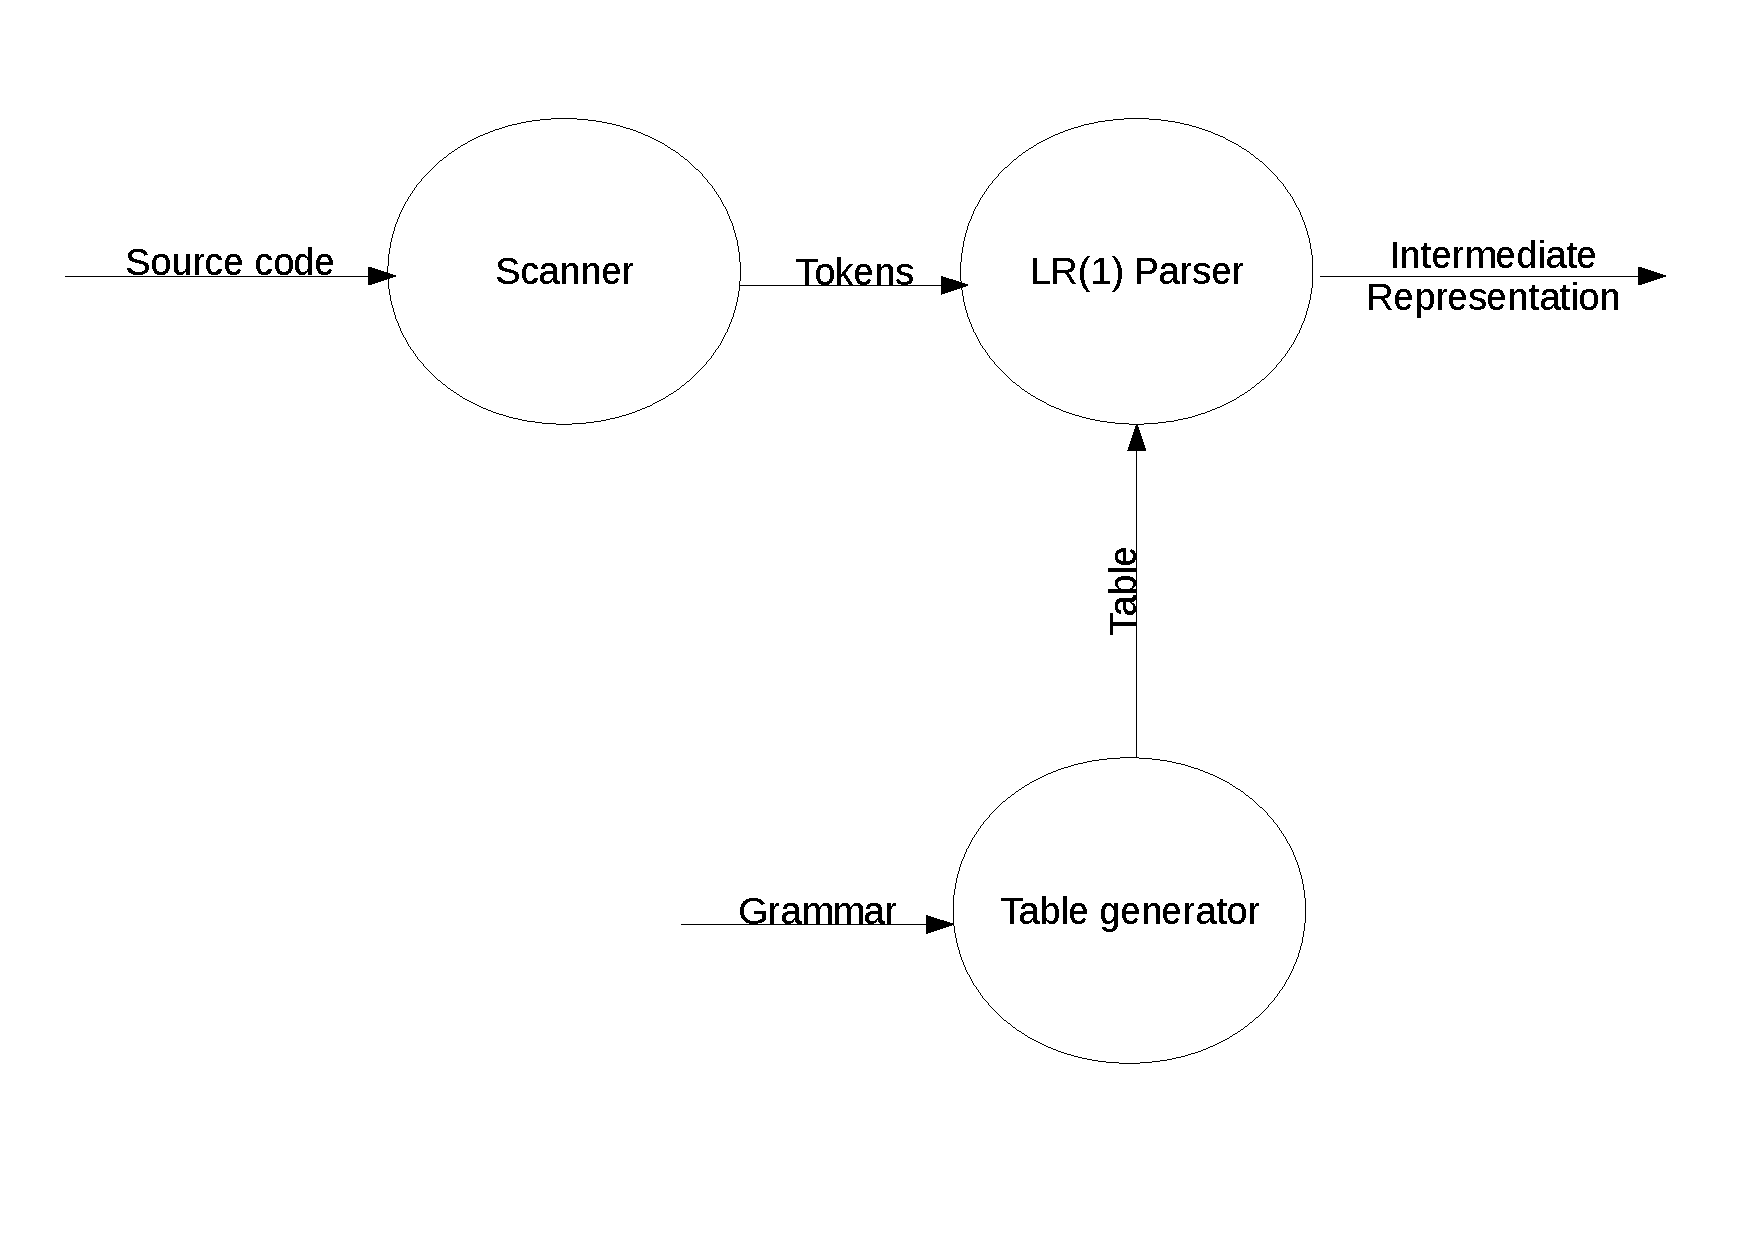
\includegraphics[width=\textwidth]{diagrams/big-picture-1}
  \caption{A diagram of the overall compiler system.}
\end{figure}

% Lecture 10

% Questions lecture, no content

% Lecture 11

\section{Context sensitive analysis}

Lexical and syntactical analysis ensure that the input program is a
valid sentence in the source language, yet though we have a parse tree
of the input program, there are still classes of errors that could be
present in the program. Since syntax analysis is context-free, any
semantic errors\footnote{These could include type errors, array index
out of bound errors (that can be detected at compile time), undeclared
variable errors etc} would not have been checked for, and would still
exist in the IR.

\subsection{Type Systems}

We can use a type system to detect many semantic errors in the
program. This involves using a \textit{type checker} to assign or
infer types for expressions and check that they are legal within
context in which they are used.

Type systems consist of a number of built in types (primitives such
as \texttt{int}, \texttt{boolean} etc, and language types such as
Java's \texttt{String}), and rules to construct new types, determine
if types are equivalent, infer\footnote{If a language requires
variables to be declared with a type before use (e.g. Java) then
inference isn't difficult. It's only when variables can be declared
as needed like in Python that it is really hard.} the type of some
expression etc. The extent of which type checking is performed varies
by language; some languages such as Java employ static type checking
at compile time, while others such as Python employ dynamic run-time
checking.

A compiler designer must consider that types affect each other; for
example, if a double is added to an int, then the result in most
programming languages would be a double.

In order to perform context-sensitive analysis, formal methods such as
grammars can be employed, ad-hoc methods are most effective (symbol
tables, syntax directed translation with attribute grammars, etc).

\subsubsection{Attribute Grammars}

Knuth had the idea to annotate each symbol in a grammar with a set of
attributes, and associate semantic rules with each production rule in
the CFG to define each attribute in terms of other attributes. We can
associate commands/actions with each rule, like so:

\begin{center}
  \begin{tabular}{>{$}l<{$} >{$}l<{$}}
    G \rightarrow E & print(E.val)\\
    E \rightarrow E_1 + T & E.val = E_1.val + T.var\\
    \phantom{E \rightarrow}~| T & E.val = T.val\\
    T \rightarrow T_1 * F & T.val = T_1.val * F.val\\
    \phantom{T \rightarrow}~| F & T = F.val\\
    F \rightarrow integer & F.val = integer.lexval
  \end{tabular}
\end{center}

% TODO: Add diagram (tree from slide 7, lecture 11) when can be arsed.

There are two types of dependencies between attributes, synthesised
dependencies and inherited dependencies. The former derive their value
from constants and their children and grammars consisting of only
synthesised dependencies can be parsed in a single bottom up pass. The
latter are inherited dependencies, and these derive their value from
their parents, siblings and constants.

An example of an inherited dependency would be parsing the
expression \texttt{int i;}, since the variable $i$ derives its type
from the symbol $int$, which would be a sibling in the parse tree.

% TODO: Look at example on page 10 on bigger screen

In order to evaluate the attributes of a parse tree, a dependence
graph must be created. Nodes represent attributes, and edges represent
the flow of the attribute values. The graph can be built as the parse
tree is built, so this isn't too expensive (and the graph is
proportional to the size of the tree too). A topological sort (nodes
are visited such that edges go from earlier to later nodes) can be
used to find independent values and use them to calculate other
values, though cyclic graphs mean that this doesn't work.

Generic attribute are rarely used in practice because lots of
supporting rules are needed. They have seen use in things like XML
editors though. Instead, a simplified idea is used; S-grammars (only
use synthesised attributes) or L-grammars (limit the use of inherited
attributes).

% TODO Read Dragon book & show an example of an S-attribute and
% L-attribute grammar.

% Lecture 12

\section{Intermediate Representation}

The intermediate representation (IR) encodes the knowledge about the
program that the compiler has derived. The purpose of an IR is to
enable retargeting for different machines (you don't have to re-write
the front end of the compiler every time), and to let machine
independent optimisations be implemented.

Things that are hard to 'get right' with IR's include the level of
abstraction that they exist on and how easy they are to manipulate and
generate. Common IR choices include a directed acyclic graph (DAG),
trees, or linear code (such pseudo code for an abstract machine). It
is emphasised in the notes that there is no unversally good choice,
and the goals of the compiler dictate what choice is best.

We can use an abstract syntax tree as an IR, and as such we want to
convert a parse tree (from the front end of the compiler) to an AST. A
parse tree contains lots of information that is not needed by the back
end of the compiler, such as that of the terminal symbols from the
CFG. The conversion involves traversing the parse tree in a post order
manner, and matching each action (in the output) with a grammar rule.

% TODO: See Aho1 pp.288-289; Aho2, 5.3.1 here

Essensially what we end up with, is the parse tree with all
non-terminal symbols removed. This is a near-source-level
representation. In fact, to generate something similar to the original
source code, then an in-order walk can be performed on the
tree. Disadvantages of AST's like this are that they're very pointer
intensive and often have multiple ways of being encoded for the same
tree.

A DAG can be used instead of an AST. These are often more powerful
than AST's, but are also harder to transform and are not useful for
showing control flow. To construct a DAG, do the same as you would for
an AST (post-order traversal \& generate nodes for each action), but
nodes can have multiple parents according to what other nodes make use
of their result.

Other graph representations include control flow graphs (each node is
a block of code, edges transfer control between them), data dependence
graphs (nodes are program statements, edges join nodes if they one
uses another's results), and call graphs which show the dependencies
between different procedures.

% TODO: Data dependence graph, control flow graph, call graph examples

\subsection{Linear Representations}

Three address code is similar to assembly, where each line is an
instruction followed by up to three operands. The code is compact,
resembles that produced as target code on many machines, and makes
intermediate values created within a computation explicit.

Each instruction in two address code only takes two operands is more
compact than three address code, but one address code (also called
stack machine code, and used by Java bytecode) is the most
compact. Each operation takes only one operand, and if more operands
are required for an instruction, then they can be popped off a stack.

\section{Back-end Datastructures}

Representing the source code as a graph/tree/stack machine translation
is useful, but we still need to encode much of the contextual
information we derived about the program. This usually includes a
symbol table (among other things), which contain a piece of code for
every production rule that is ran when the production rule is
applied. Examples of code could be to type check an assignment, or
check that a variable has been declared before it it used. Symbol
tables are retained between multiple compilations (and also during
debugging) so that they do not have to be re-constructed each time.

Things that go inside a symbol table include variable names,
constants, function names, strings, text labels, and temporary
variables for the compiler. The actual information stored about each
entity varies according to what the entity actually is. Quick access
is important, since the symbol table is frequently accessed by the
compiler.

Obviously you could implement a symbol table in a variety of ways, but
a hash table is most commonly used due to its $O(1)$ lookup time
(linked lists or binary trees are worse alternatives). In the course
notes, bucket hashing is mentioned to resolve hash collisions, where a
linked list is maintained for each hash value to store items with that
hash key. Open addressing is also given, which is where the hash value
is recalculated with an added constant each time there is a collision
until a free space is found.

% Lecture 13

\section{The Procedure Abstraction}

The front end of the compiler is well understood and theoretically
sound, while the second half is a more hotch-potch affair; it is here
that clever engineering must by used to solve NP-hard problems and
choose between diffucult trade offs.

Programming is all about abstraction, and one of the main tools in a
programmer's abstraction toolbox is the procedure. Procedures let
programmers define entry and exit points to a block of code, work
within a set context, and have a clean external interface that can be
used to call the code. However, there must be an agreement between
different parts of the system as to how procedures are to work; how is
memory laid out (and protected), how are arguments passed, where are
procedures stored, etc. These concerns transcend those of the
compiler, the Operating System, and to an extent, the architecture of
the machine must all be designed with this in mind.

Sometimes each procedure is compiled individually, meaning that the
compile time can be reduced (less code in each procedure means less
complexity for the compiler, and recompilation needs only to concern
the procedures that have been edited).

\subsection{Linkage}

Since procedures have such well defined control flow behaviour, a
protocol exists for passing values and control at procedure calls and
returns. This is called the linkage convention, and it ensures that
procedures inherit a valid run-time environment and that they restore
one for their parents.

The code to make a linkage happen is generated at compile time, but
generated at runtime. To do this, the compiler must consider that
local variables require storage during procedure execution, and it
must set asside a region of memory for this (and other things) called
an activation record (AR)\footnote{They are called activation records
in the notes, but are referred to as stack frames in most places I've
seen.}. Things stored within the AR include:

\begin{itemize}
\item Parameters to the function
\item Register save area
\item Return value
\item Return address
\item Access link (helps with non-local access)
\item Caller's access link (to return to parent once complete)
\item Temporary variables and local variables
\end{itemize}

This is how the whole process happens, and what each part is responsible for:

\begin{itemize}
\item Caller (pre call)
\begin{itemize}
\item Allocate the AR
\item Store the parameters in the AR
\item Store the return address
\item Jump to the child
\end{itemize}
\item Callee (prologue)
\begin{itemize}
\item Save the caller's registers
\item Extend the AR for local data
\item Init local variables
\item Start execution
\end{itemize}
\item Callee (epilogue)
\begin{itemize}
\item Store the return value
\item Restore registers
\item Unextend the AR frame
\item Jump to return address
\end{itemize}
\item Caller (post return)
\begin{itemize}
\item Copy the return value
\item Deallocate the caller's AR
\item Restore the parameters
\end{itemize}
\end{itemize}

At runtime, the size of the code and static/global variables are
known, but the size of the heap and stack varies. As such, the address
space is organised like so:

\begin{figure}[H]
\centering
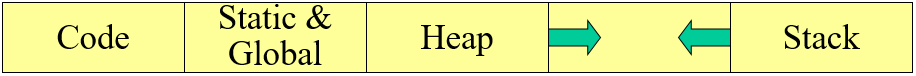
\includegraphics[width=\textwidth]{diagrams/memory-layout}
\caption{\label{fig:memory-layout}The memory layout of a program. The
heap and stack grow towards each other.}
\end{figure}

Variables are stored in the AR using offsets, but must be put on the
heap if the variables themselves are of variable length. The
activation records themselves will either be on the heap or the stack;
if the procedure makes no calls, then the AR can be allocated
statically, if it has a normal return value, then it can simply go on
the stack as normal (which is good, because we don't need to worry
much about deallocation), but if it may need to be active after exit
(e.g. it returns a pointer pointing to a local variable), then it
should be on the heap. The heap is least efficient, the stack is more
efficient, but static allocation is most efficient.

Most variables are allocated at runtime, but static and global
variables are usually allocated at compile time since their memory
requirements are known inadvance. Variables can either be put on the
stack or on the heap, and are done so according to whether they need
to be preserved across procedures and if they have fixed sizes.

% TODO: Bit about addressing variables missed out (slides 10->13 in slides)

The compiler must consider things like storing variables at the start
of word boundaries and re-ordering variables to maximise memory usage
efficiency. The proximity and ordering of variables can also affect
cache performance (they are likely to be fetched in the same cache
load). The compiler can also avoid some problems/overheads relating to
procedure calling/linkage by inlining procedures (copying their code
into another procedure with no call), though this is not possible in
all cases due to register consumption, code size (too many inline
functions means lots of repeated code), cache trashing etc.

% Lecture 14

% Questions lecture, no content

% Lecture 15

\section{Code generation \& instruction selection}

Here, we want to map the IR to low level machine instructions. The
compiler also needs to make sure that the generated program stays
within the resource limits of the CPU; different processors have
different amounts of registers for example. Accessing data in
registers is of course far more efficient than having to access data
in memory, so intelligent use of registers (register allocation) is
important for efficiency.

It is here that compilers apply tricks such as instruction reordering,
where operations are re-ordered to hide latencies in other
operations. Instruction selection, register allocation and instruction
scheduling are all NP-complete problems that can be solved
independently\footnote{For example, instruction reordering can happen
at a higher level than register allocation, for example whole program
statements (that compile down to hundreds of instructions) can be
reordered, but there is no equivalent for register allocation.}.

We are using a very simple instruction set; \texttt{LDR RX, ADDR/RY}
(with direct \& indirect addressing), \texttt{MOV RX, RY}, \texttt{ADD
RX, RY, RZ}, \texttt{SHR RX, RY, VAL}, \texttt{STORE RX}. However,
instructions have different \textit{latencies}\footnote{The time (in
cycles) between the instruction being issued and the time that the
instruction results can be used.}, which the compiler needs to take
into account.

\subsection{Generating code for arithmetic expressions}

% Slide 5

We can simply walk the IR in postorder and generate code with a
procedure like this:

% TODO: Put in code generating procedure

% TODO: Talk about choosing what operations to implement first (slide
% 6)

On most processors, the cost of multiplication might be several
cycles, while shifting and adding is typically one or two cycles. In
many instances, we can use shifting and addition instead of
multiplications, so that we can multiply some constant integer with an
unknown integer efficiently\footnote{Like in COMP27112}.

\subsection{Trading register usage with performance}

Often, if we load values into registers first and compute after, then
we can hide some of the memory latency. However, doing this uses up
registers, of which we have a finite limit.

% TODO: Example from slide 8

\subsection{Array references}

The compiler must always use the same storage scheme for arrays;
either row-major order, column-major order or indirection orders (each
element is a pointer to the actual array value).

% TODO: Talk about finding the correct offset for an index.

\subsection{Boolean \& relational values}

The compiler can use a treewalk generation like with arithmetic
expressions...

% TODO: Slide 10

\subsection{Control flow statements}

% TODO Slide 11

% TODO Slide 12; conclusion

% Lecture 16

\section{Register allocation}

The compiler must choose what registers to store data in while the
program is executing. We assume that a three-address code has been
generated, which uses an unlimited abount of \textit{virtual
registers}, but we want to map that onto the \textit{phyiscal
registers} in the machine.

Henceforth, the task is to produce correct code that uses at most $k$
registers, and minimises the number of loads and stores to memory
(i.e. minimise register spilling). Ideally, we don't use backtracking
so the compiler is fast.

\marginpar{It is important to remember that real processors have many
different register types, and real compilers must factor this in when
allocating.}A \textit{basic block} is a segment of branch-free,
straight line code. Local register allocation is within a basic block,
and global allocation is within an entire
procedure. \textit{Allocation} is choosing what values to keep within
registers, but \textit{assignment} is choosing which specific
registers get the values.

To determine how many registers we need in a given basic block, we
must compute a set of \textit{live ranges}, where the value of a
variable is live between its definition and its last use. We must
define a value \texttt{maxlive} to be the maximum number of live
variables we can have in registers, and if the number of live ranges
active at any point is greater than this value, then the registers
must spill to memory.

A common top-down method of register allocation is
the \textit{frequency count algorithm}, where $f$ registers are
reserved for use when loading and saving values to memory, and so
$k-f$ registers are used for the program. The compiler looks at the
$k-f$ most commonly used values and stores them in registers, while
using the $f$ registers to spill the other values to memory.

Bottom up register allocation uses \textit{Best's algorithm}, which is
given as:

\begin{verbatim}
for (op, vr3, vr2, vr1) in operations
  ensure vr1 in r1
  ensure vr2 in r2
  if r1 not needed after this instruction
    free(r1)
  endif
  if r2 not needed after this instruction
    free(r2)
  endif
  allocate r3 for vr3
  emit op r3, r2, r1
\end{verbatim}

This relies on two operations; \textit{ensure}
and \textit{allocate}. The former assigns a virtual register to an
actual register and ensures all occurances of that virtual register
are tied to the real one. The latter allocates a free physical
register, or finds the register that is being used farthest in the
future, stores its value and returns it.

In practice, we often have multiple basic blocks being executed one
after the other, and there are often opportunities for optimisation
between them (e.g. some basic blocks use values already in the
registers of others). If the control path between the basic blocks is
nonlinear, then this may not be easy.

Rather than looking at local blocks of code in isolation, some
approaches take the global program into account, and use generalised
frequency counts as well as avoiding load and store operations between
different basic blocks. Graph colouring can be used to assign
registers if each colour is mapped onto a register.

% Lecture 17

% Lecture 18 (Instruction scheduling)

\section{Instruction Scheduling}

The problem of instruction scheduling is that given some target code,
the latencies for each operation on the target machine, we need to
reorder operations in order to minimise the execution time of the
code. This is made more complicated by the fact that modern processors
usually have multiple functional units.

More specifically, we want to produce correct code (most importantly),
minimise the number of wasted CPU cycles, avoid spilling registers and
to operate efficiently (depending on your definition of efficiency).

Many CPU instructions have some delay latencies for execution, memory
operations in particular. Modern processors issue several operations
per cycle, and the execution time of each is often order dependent. In
order to minimise waiting for load operations, we can move them back
so that their data becomes available when it is needed, but this
increases register pressure. The general idea is to do things that are
potentially costly as early as possible so that the result is likely
to be ready for when it is needed.

% We can put a motivating example here. (e.g. slide 3)

\subsection{Instruction Scheduling - How To}

% TODO: Check
Instruction Scheduling is NP-Complete, so we use heuristics to do it as best as we can.

\begin{itemize}
        \item Build a precedence graph (of data dependencies)
        \item Compute a priority function for the nod esof the graph
        \item Use list scheduling to construct a schedule, one cycle at a time:
        \begin{itemize}
        \item Have a queue of ready operations
        \item At each cycle, choose an operation from the queue and execute
        it (and update the ready queue according to the dependencies in the precedence graph).
        \end{itemize}
\end{itemize}

This is a greedy heuristic, and can (obviously) be modified. The
priority function really determines what instructions are scheduled
first among the ready instructions. One example priority function
could be $p(node) = latency(node) + max(p(child\#1), p(child\#2),
\dots, p(child\#n))$.

% TODO: Example

\subsection{List scheduling}

% TODO: Add content from slide 5-9

\begin{tabular}{lll}
Ready & Scheduled & Active\\ \hline
6,4,1,3 & 6 & 6\\ \hline
1,4,3 & 1 & 6, 1\\ \hline
2,4,3 & 2 & 6, 2\\ \hline
4, 3 & 4 & 6,4\\ \hline
3,7 & 7 & 7,4 \\ \hline
% TODO fill in from slides
\end{tabular}

There are two distinct classes of list scheduling, forward list
scheduling and backward list scheduling. Forward scheduling starts
with the available operations and works forward in time, but backward
scheduling starts with the leaves and works backwards in time (using
latency to determine what is available). Often both are applied and
whichever produces the best result is used.

The priority function has many variations, including prioritising the
critical path, prioritising nodes with many immediate successors or
total number of descendants, ignoring latency etc

\subsection{Multiple functional units}

When we have multiple functional units, we just run the list
scheduling algorithm as normal, but have it schedule multiple
operations (as many as we have functional units) per cycle.

% TODO: Give example w/ 2 functional units

\subsection{Further issues}

We want to identify highly used sections of code and spend more time
optimising that (or schedule it as a single block). We can also
schedule multiple loop iterations together (loop unrolling) so that we
can reduce the overhead of the loop. Register allocation can restrict
the choices for instruction scheduling (not enough registers), so
optimising allocation to avoid spilling (loading and storing to
memory) is beneficial. We also want to minimise the size of the code
and the energy usage of the code.

% Lecture 19 (last one!)

\section{Code optimisation}

Code optimisation is very hard and could be a course on its own. The
end goal is to improve the performance of the program within some
constraints, for example, to reduce the size of the code, improve the
performance, reduce memory bandwidth, reduce power consumption etc.

The issues are the legality (the meaning of the program must be
preserved), benefit (we need to optimise for the average or common
case, but determining what these cases are is often non-trivial) and
compile time cost (there are a large number of possible optimisations,
applying them all takes a long time).

Optimising transformations can be applied at multiple levels of
abstractions; at the source code level (choosing the right algorithm),
at the IR level (machine independent) and at the target code level
(machine-dependent). Typical transformations include discovering and
propagating constant values, removing unreachable code or redundant
computations, or encoding a computation in some particularly efficient
form.

We can classify optimisations by their scope (local (within a block),
peephole (within a few blocks), loop level, global, inter-procedural
(across a whole program or between procedures)), by machine
information (such as machine dependent or independent operations) or
by their effect on the structure of a program (e.g. re-ordering
algebraic operations).

Examples of transformations applied for optimisation purposes include:

\begin{tabular}{>{\bfseries}p{0.2\textwidth}p{0.4\textwidth}p{0.4\textwidth}}
Name & \textbf{Before} & \textbf{After}\\ \hline

  Computing common subexpressions &
  \texttt{A[i, i * 2 + 10] = B[i, i * 2 + 10] + 5} &
  \texttt{tmp = i * 2 + 10}\newline
  \texttt{A[i, tmp] = B[i, tmp] + 5}\\ \hline
  
  Copy propagation &
  \texttt{t = i * 4}\newline
  \texttt{s = t}\newline
  \texttt{a[s] = a[s]+5} &
  \texttt{t = i * 4}\newline
  \texttt{a[t] = a[t]+5}\\ \hline

  Constant propagation &
  \texttt{N = 64}\newline
  \texttt{c = 2}\newline
  \texttt{for (i = 0; i < N; i++) }\newline
  \texttt{a[i] = a[i] + c}\newline
  \texttt{}&
  \texttt{N = 64}\newline
  \texttt{c = 2}\newline
  \texttt{for (i = 0; i < 64; i++)}\newline
  \texttt{a[i] = a[i] + 2}\newline
  \texttt{}\\ \hline

  Constant folding &
  \texttt{tmp = 5 * 3 + 8 - 12 / 2} &
  \texttt{tmp = 17}\\ \hline

  Dead code elimination &
  \texttt{if(3>7) {...}} &
  \texttt{// Nothing}\\ \hline

  Reduction in strength &
  \texttt{y = x * 2 + x * 1024} &
  \texttt{y = x + x + (x<<10)}\\ \hline

\end{tabular}

\subsection{Loop optimisation}

Loops are an important target for optimisation, mainly because much of
the complexity inherent in programs is derived from looping control
structures. Three optimisations are mentioned in the course:

\begin{description}
  \item \textbf{Loop-invariant code-motion}:\\ If a constant
    expression is computed inside a loop, move the computation outside
    the loop so that it is only done once.
    
  \item \textbf{Loop interchange}:\\ Swap the variables that are being
  altered in two nested loops so that the order of access matches the
  order that the data items are in memory. The course notes describe
  the aim as being to achieve `unit stride' accesses, i.e. so that
  each access is one sequential array stride from the last.

  \item \textbf{Strip mining}:\\ Strip mining transforms a singly
  nested loop into a double nested one. The outer loop steps through
  the index in blocks of some size, and the inner loop steps through
  each block. The block size of the outer loop is determined by some
  characteristic of the target machine, such as the vector register
  length or the size of one cache line.

  \item \textbf{Loop unrolling}:\\ The idea behind loop unrolling is
  to process multiple iterations of the loop inside one iteration to
  reduce the overhead of looping and perhaps make better use of SIMD
  instructions or to make scheduling easier. For example:
  
  \begin{verbatim}
    for (int i = 0; i < 12; i++) x[i] += 1;
  \end{verbatim}

  Could go to:

  \begin{verbatim}
    for (int i = 0; i < 12; i+=4) {
      x[i] += 1
      x[i+1] += 1
      x[i+2] += 1
      x[i+3] += 1
    }
  \end{verbatim}

  Or even:

  \begin{verbatim}
    // Add8 does four 8-bit add operations in one instruction
    for (int i = 0; i < 12; i+=4) add8(x[i], 1);
  \end{verbatim}

  If the number of loop items is not divisible by the unroll length
  (four in our case), then an additional loop may be added after the
  main loop to complete the last few iterations.
\end{description}

Asserting that these optimisations are legal is a hard problem. A
model is often used to represent the loop control logic, by which
logical conclusions can be drawn. The main issue is data dependence;
in order to do things like switching an inner and outer loop, we need
to ensure that the end result is the same if the loops interact with
each other.

